99. а) $f(x)=\begin{cases} |x-3|-4,\ x>1\\ -x^2-3x+4,\ x\leqslant 1\end{cases}$
$$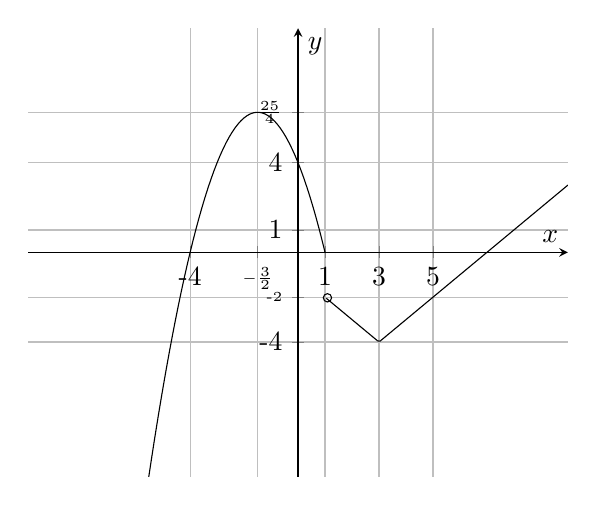
\begin{tikzpicture}[scale=1]
\tikzset{line03/.style={dashed,line width =0.9pt}}
\begin{axis}[
    axis lines = middle,
    grid=major,
    legend pos={south west},
    xlabel = {$x$},
    %xlabel style={below right},
    ylabel = {$y$},
    ymin=-10,
    ymax=10,
    xmin=-10,
    xmax=10,
    xtick={-4, -1.5, 1, 3, 5},
    xticklabels={-4, \tiny{$-\frac{3}{2}$}, 1, 3, 5},
    ytick={6.25, 4, -4, 1, -2},
    yticklabels={\tiny{$\frac{25}{4}$}, 4, -4, 1, \tiny{-2}},        ]

	\addplot[domain=1.05:10, samples=100, color=black] {abs(x-3)-4};
	\addplot[domain=-10:1, samples=100, color=black] {-x*x-3*x+4};

\end{axis}
\draw  (3.8,2.27) circle (1.5pt);
%\draw[line03] (3.11,0) -- (3.11,6);
%\draw[line03] (0,3.7) -- (6.5,3.7);
%\draw (3,5.7) node {\scriptsize $y$};
%\draw (7,2.5) node {\scriptsize $x$};
\end{tikzpicture}$$
б) По графику определим, что горизонатльная прямая $y=\cfrac{a}{2}$ пересекает график функции $f(x)$ дважды в следующих случаях:
$\cfrac{a}{2}=-4,\ \cfrac{a}{2}=\cfrac{25}{4}$ или $\cfrac{a}{2}\in[-2;0),$ таким образом $a\in\left[-4;0
ight)\cup\left\{-8;\cfrac{25}{2}
ight\}.$\\
